% File example.tex
% Contact: simonnet@ecole.ensicaen.fr
%
% version 1.0 (July 24, 2009)
% version 1.1 (September 3, 2009)
% add using of the optional command: \secondauthoraddr



\documentclass[10pt]{article}

% File icdp2009.sty
% Preamble that you have to include to use the template  

% July 24, 2009
% Contact: simonnet@ecole.ensicaen.fr


\usepackage[a4paper,textwidth=18cm,textheight=24cm,top=2.85cm, bottom=2.85cm, left=1.5cm, right=1.5cm]{geometry}

\usepackage{template/icdp2009}

% left justified caption
\makeatletter
\long\def\@makecaption#1#2{%
\vskip\abovecaptionskip
\sbox\@tempboxa{#1. #2}%
\ifdim \wd\@tempboxa >\hsize
#1. #2\par
\else
\global \@minipagefalse
\hb@xt@\hsize{\box\@tempboxa\hfil}%
\fi
\vskip\belowcaptionskip}
\makeatother




%other package
\usepackage{amsmath}

% vectorial font
\usepackage{lmodern}

\usepackage{graphicx}
\usepackage{times}


\begin{document}
\noindent

\bibliographystyle{plain}

\title{K-Nearest Neighbours Classifier\\Assignment 3 of Machine Learning I, 2022/2023}

\authorname{Mura Alessio}
\authoraddr{DIBRIS - Dipartimento di Informatica, Bioingegneria, Robotica e Ingegneria dei Sistemi\\
Università Degli Studi di Genova}

% \secondauthoraddr{+Affiliation,Country and contact details }


\maketitle

% % \keywords
% % Maximum 5 keywords placed before the abstract.

% \abstract
% This is where the abstract should be placed. It should consist
% of one paragraph and a concise summary of the material
% discussed in the article below. It is preferable not to use
% footnotes in the abstract or the title. The acknowledgement
% for funding organisations etc. is placed in a separate section at
% the end of the text. We wish you success with the preparation
% of your manuscript.

\section{Introduction}
Classification in machine learning and statistics is a supervised learning approach in which the computer program learns from the data given to it and makes new observations or classifications.
\\\\One of the most common classifier is the \textbf{k-Nearest Neighbour
classifier [KNN]}. KNN is a supervised learning algorithm that estimates how likely a data point (instance) belongs to one class or the other depending upon which class its ‘k’ nearest instances belong to. \\\\It is a non-parametric model that means it does not make assumptions about the data pre-hand like they do in case of linear regression that the data must linear. KNN is referred to as a \textit{Lazy Learner}, because it does not really do anything during the training phase, actually, there is no as such a training phase for KNN, means it does use the training data points to do any kind of generalization

\section{Theory of KNN Classifier}
Given an input point $\bar{x}$ called \textit{query}, the goal is to classify
this point using all the other points that surrounds it. The
classifier then gives the predicted class $\omega$ as output, such that
$\omega$ = \textit{y($\bar{x}$)}, where \textit{y()} is the rule of the kNN.
\\\\The decision rule is based on the concept of the \textbf{majority voting}, meaning that the $\bar{x}$ will be classified with the class
$\omega$1 only if the majority of the k-closest objects around him belongs to the class $\omega$1.
\\\\Let’s define X as the training set given as input to the kNN:
\begin{equation}
    X =\begin{bmatrix}
            x_1\\
            x_2\\
            .\\
            .\\
            x_n\\
        \end{bmatrix}
\end{equation}
where $x_i$ is a single observation of the training set. \\\\\\\\\\\\The k-Nearest Neighbour classifier computes the \textit{distance} (norm) between each observation $x_i$ and the query point $\bar{x}$, and stores it in a row vector \textbf{N}:
\\\\
\begin{equation}
    N =\left( \lVert x_1 - \Bar{x} \rVert, \lVert x_2 - \Bar{x} \rVert,..., \lVert x_n - \Bar{x} \rVert\right)
\end{equation}
where each value stored inside \textbf{N} tells how much the query point is similar to the considered observation.\\\\
The kNN classifier than takes into account the first k points
that are closest to $x_i$ (i.e. the k points that are most similar to
the query one)
\begin{equation}
     \bigl\{ n_1,...,n_n\bigl\} = top_k\lVert x_i - \Bar{x} \rVert
\end{equation}
The class given to $x_i$ is then the class that appears the most:
\begin{equation}
     \omega = \textit{mode}\bigl\{ t_n_1,...,t_n_k\bigl\}
\end{equation}
where $t_n_1$ is the class of the class 1.
\\\\
Moreover, it is possible to visualize the performance of our prediction model by a \textbf{Confusion Matrix}.
\\\\
A Confusion matrix is an $N x N$ matrix used for evaluating the performance of a classification model, where N is the number of target classes.
It can be used to evaluate the performance of a classification model through the calculation of performance metrics like accuracy, precision, recall, and F1-score. 
\\\\
In our case, we used a Confusion Matrix for Multi-Class Classification in order to check the performance for each digits.
\newpage
\section{THE ASSIGNMENT}
The given assignment consist of three tasks:
\begin{itemize}
 \item \textbf{Task 1}: Obtain a data set
 \item \textbf{Task 2}: Build a kNN classifier
 \item \textbf{Task 3}: Test the kNN classifier
 \end{itemize} 

\subsection{Task 1: Obtain a data set}
This assignment takes into account the MNIST set, a standard benchmark for machine learning tasks. \\The data represent 70000 handwritten digits in 28x28 greyscale images, already split into a 60000-image training set and a 10000-image test set, 784 attributes and 10 classes.\\\\
Since the two sets are very big, two random subsets are selected inside the main function [600 for training set and 100 for the test set].
By using Python solution, the machine learning library \textit{keras}, part of \textit{tensorflow}, contains ready-made functions. Just do the following:
\begin{center}
    from tensorflow.keras.datasets import mnist
    $\left( train_X, train_Y\right), \left( test_X, test_Y\right) = mnist.loadData()$
\end{center}

\subsection{Task 2: Build a kNN classifier}
In the second tasks, we have to actually implement a k-Nearest Neighbour classifier. In order to check the correctness of the input variables, we created some functions: \textit{CheckDataset()}, \textit{Check-K-value()}.
\\\\
Subsequently, we classified the dataset
according to the kNN theory, described with formulas 2, 3 and 4, and returned the classification obtained.
\\\\
We computed the classification by a function we created: \textit{KNNclassifier()}. After applying the reshape function, in order to work in 2-Dimensions, and initilizing the lists, we computed a prediction list and stored it into a dictionary. Then we sorted in ascending order by \textit{Euclidean distance} and got the count of the maximum class in result list.
\\\\
Finally, we computed the accuracy and error rate by checking if the values inside pred-list were equal to test-y.
The function returns: accuracy, error rate and pred-list.




\subsection{Task 3: Test the kNN classifier}
In task 3 it is required to run the kNN classifier using different values of k. The values used are:
\begin{center}
    $K_1 =\bigr[1,2,3,4,5,10,15,20,30,40,50\bigr]$ 
\end{center}
By a \textit{for loop}, we passed each of the previous k-value inside \textit{KNNclassifier()} and plotted the respective results in a subplot graph where we reported the accuracy and error rate.
\\\\
Then, we created a \textbf{Confusion Matrix} by some functions: \textit{ConfusionMatrix()} and \textit{ClassificationQualityIndexes()}.
First of all, we created a matrix $10x10$ (10 is the number of digits) and computed all the quality indexes by the following four terminologies:
\begin{itemize}
 \item \textbf{True Positives (TP)}: when the actual value is Positive and predicted is also Positive.
 \item \textbf{True negatives (TN)}: when the actual value is Negative and prediction is also Negative.
 \item \textbf{False positives (FP)}: When the actual is negative but prediction is Positive.
 \item \textbf{False negatives (FN)}: When the actual is Positive but the prediction is Negative.
 \end{itemize} 
 \\
 In order to have a clear representation of the performance, we reduced the set of k value:
 \begin{center}
    $K_2 =\bigr[1,3,5,10,25,50\bigr]$ 
\end{center}
\\
Finally, we compared the accuracy of the classifier on the different classes (i.e. digits), checking each digit vs the
remaining nine,  by repeating the previous steps.

\section{RESULTS}

\begin{figure}[h] 
	\centering
	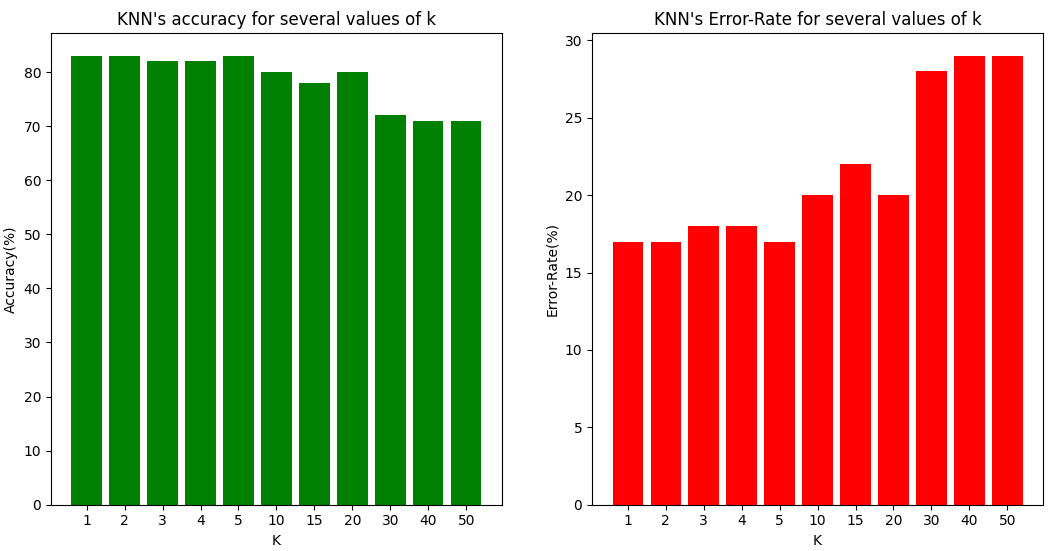
\includegraphics[width=0.9\columnwidth]{Figure_1.png} % Example image
	\caption{Accuracy and Error rate for several values of k.}
\end{figure}

\\
As shown in Figure 1, the error rate increases as the value of k gets higher. The best value of k should then be lower then 10, in order to avoid taking considering some wrong neighbours.

\begin{figure}[h] 
	\centering
	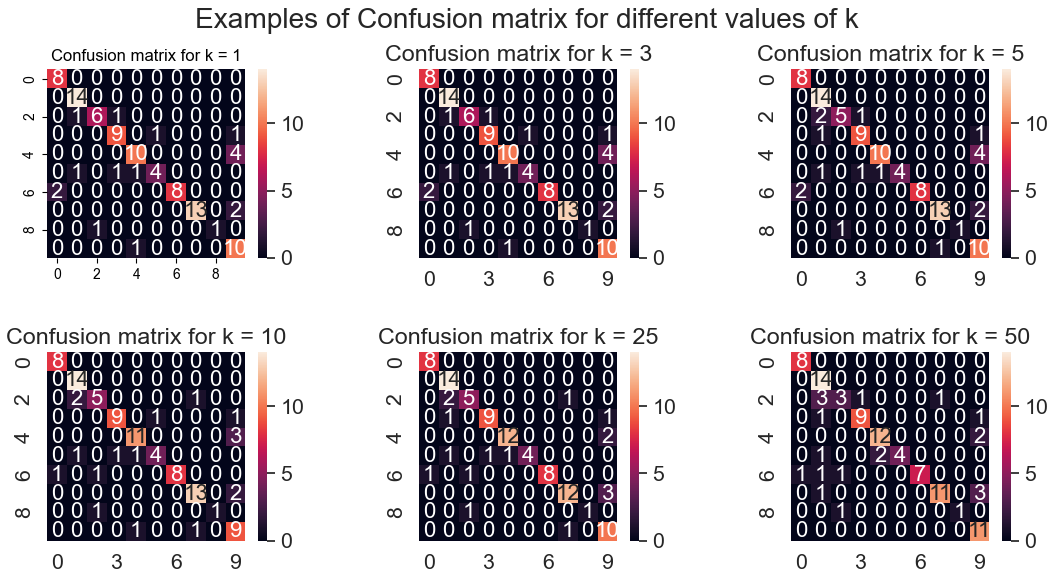
\includegraphics[width=0.9\columnwidth]{Figure_2.png} % Example image
	\caption{Confusion matrix for different values of k.}
\end{figure}
\newpage
As shown in Figure 2, we can clearly see that the higher values are along the diagonal. This agrees with the theory, because the cells along the diagonal represent the \textbf{True Positives (TP)} values, that is when the actual value is well predicted.

\begin{figure}[h] 
	\centering
	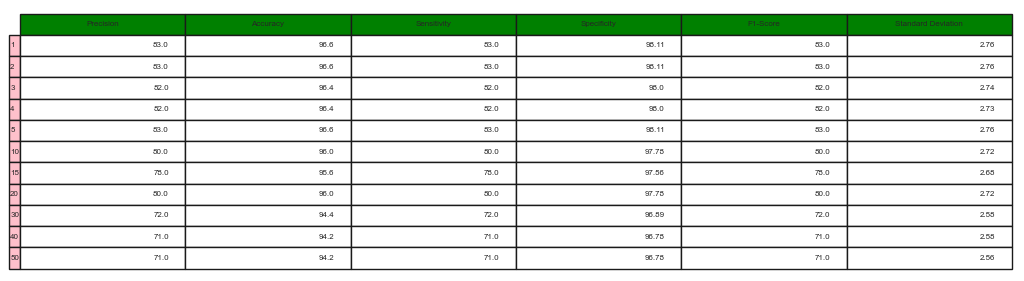
\includegraphics[width=1.0\columnwidth]{Figure_3.png} % Example image
	\caption{Quality indexes for different values of k.}
\end{figure}

First of all, we have to define what each Index means:

\begin{itemize}
 \item \textbf{Precision}: It is a measure defined as the ratio of the total number of correctly classified positive classes divided by the total number of predicted positive classes.
 \item \textbf{Accuracy}: It is a measure defined as the ratio between the number of correct predictions and the total number of predictions.
 \item \textbf{Sensitivity}: It is a measure defined as the ratio of the total number of correctly classified positive classes divide by the total number of positive classes.
 \item \textbf{Specificity}: It is a measure that tells us what fraction of all negative samples are correctly predicted as negative by the classifier.
 \item \textbf{F1-score}: It is a number between 0 and 1 (in our case we use percentage) and is the harmonic mean of precision and recall.
 \item \textbf{Standard deviation}: It is a statistic that measures the dispersion of a dataset relative to its mean and is calculated as the square root of the variance.
 \end{itemize} 

By Figure 3, we can infer that our prediction was quite successful. Now, in a perfect world, we’d want a model that has a precision of 1 and a recall of 1. That means a F1-score of 1.


\begin{figure}[h] 
	\centering
	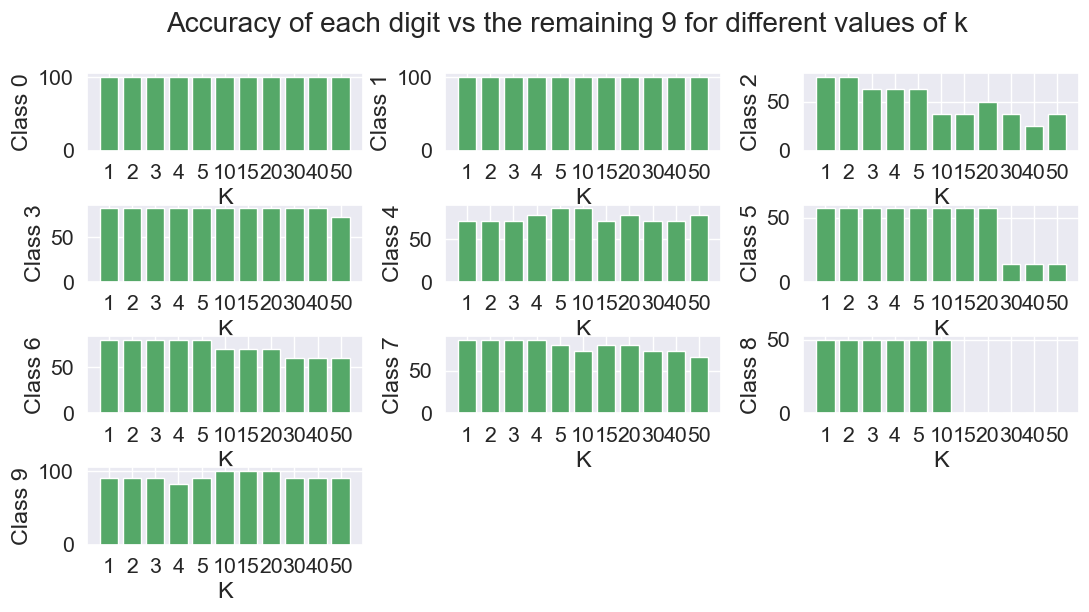
\includegraphics[width=1.0\columnwidth]{Figure_4.png} % Example image
	\caption{Accuracy for each digit vs remaining nine.}
\end{figure}

By Figure 4, It is clearly visible that the easiest classes to recognize in general are 0 and 1 (with an accuracy of 100\%), while the hardest class to recognize in general is 8 (with an accuracy of 50\%, meaning that one classification every two is wrong).
Moreover, we can see that, as the value of k gets higher, the accuracy decreases.


\begin{figure}[h] 
	\centering
	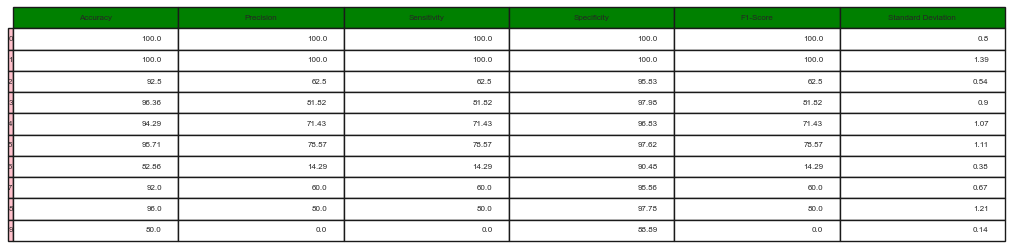
\includegraphics[width=1.0\columnwidth]{Figure_5.png} % Example image
	\caption{Quality Indexes for each digit vs remaining nine.}
\end{figure}

Finally, by Figure 5, we can infer what we got in the previous case, that is the correctness of the prediction for each digits vs the remaining nine, in the case that K was equal to 5.
\\\\
In fact, the easiest classes to recognize are 0 and 1. Whereas, with this k value, the hardest one is class 9.
\\\\
Obviously, for each value of K, the hardest class to recognize will change.


\end{document}